\documentclass[preprint,12pt,authoryear]{elsarticle}

\usepackage[T1]{fontenc}
\usepackage[utf8]{inputenc}
\usepackage{amsmath,amssymb}
\usepackage{booktabs}
\usepackage{graphicx}
\usepackage{microtype}
\microtypesetup{expansion=false}
\usepackage{multirow}
\usepackage{siunitx}
\usepackage{tikz}
\usepackage{xcolor}
\usepackage{url}
\usetikzlibrary{arrows.meta,fit,positioning,shapes.geometric}
\definecolor{TrustTeal}{HTML}{16796F}
\definecolor{TrustCharcoal}{HTML}{243746}
\definecolor{TrustAmber}{HTML}{C06B19}
\definecolor{TrustPaleTeal}{HTML}{E1F2EF}
\definecolor{TrustPaleAmber}{HTML}{FFF0DC}
\tikzset{
  trustbox/.style={draw=TrustTeal,very thick,rounded corners=2pt,fill=TrustPaleTeal,align=center,minimum height=9mm,text=TrustCharcoal},
  machine/.style={trustbox,dashed},
  human/.style={draw=TrustAmber,very thick,rounded corners=2pt,fill=TrustPaleAmber,align=center,minimum height=9mm,text=TrustCharcoal},
  fact/.style={trustbox,fill=white},
  flow/.style={-{Latex[length=2.2mm]},thick,draw=TrustCharcoal},
  noflow/.style={thick,draw=TrustAmber,densely dashed}
}

\setlength{\emergencystretch}{2em}

\journal{Expert Systems with Applications}

\begin{document}
\begin{frontmatter}

\title{Auto-Decte: Trust-Constrained Document Intelligence through Candidate--Fact Separation and Selective Prediction}

\author{Anonymous author(s)}
\affiliation{organization={Anonymous institution},country={Anonymous country}}

\begin{abstract}
Document intelligence in payroll-adjacent and production workflows must control both recognition error and the authority granted to machine output. Auto-Decte is a trust-constrained human-in-the-loop architecture for structured industrial forms. Its central invariant separates immutable evidence, append-only machine candidates, attributable human decisions, and versioned facts: perception, retrieval, and language-model services have no direct fact-writing capability through the evaluated application interfaces. We tested the implementation at three levels. First, a seed-disjoint cell benchmark evaluated 2,610 conditions derived from 90 base units. A HOG--linear-SVM recognizer achieved 99.81\% accuracy at full coverage; cluster bootstrap placed its selective-risk 95\% interval at 0.038\%--0.346\%. Second, 60 synthetic forms from two templates were evaluated under five whole-page conditions. The complete pipeline succeeded on 60\% of the 300 form--condition rows, including every clean, perspective, and JPEG row; blur prevented QR identification and rotation prevented marker alignment. Removing either QR identity or ArUco alignment reduced complete-form success to zero under an endpoint that requires both operations. Third, all 60 evidence-to-export workflows produced a versioned fact and a valid reverse trace, 12 attempted direct machine fact-write paths were unavailable, and 500 randomized fault trials left existing facts unchanged. The evidence supports the executable authority boundary and identifies concrete perception failures, but not production effectiveness: independently transcribed real forms and controlled reviewer studies remain necessary.
\end{abstract}

\begin{keyword}
document intelligence \sep human-in-the-loop \sep selective prediction \sep data provenance \sep trustworthy artificial intelligence
\end{keyword}
\end{frontmatter}

\section{Introduction}
\label{sec:introduction}

Document processing is often evaluated as a prediction problem: an image enters a model and structured values leave it. That abstraction is incomplete in payroll-adjacent and production workflows. A wrong digit may alter a wage calculation, a stale record may be mistaken for current evidence, and a plausible language-model suggestion may be granted authority that its provenance does not justify. In such settings, the consequential question is not only whether a machine output is accurate, but also whether that output can silently become an operational fact.

Modern document models substantially improve representation learning and extraction across layouts \citep{layoutlm,layoutlmv2,layoutlmv3,donut,docformer,trocr}. Human-in-the-loop systems can direct difficult examples to reviewers \citep{budd2021,mosqueira2023}, while retrieval-augmented and generative systems can supply context or candidate values \citep{gao2023,xu2024}. These capabilities solve complementary inference and interaction problems. They do not, by themselves, constrain the authority of a machine output in the application data model. A high-scoring prediction and a retrieved historical value remain unsafe if either has an unreviewed write path to an authoritative record.

We study the following question: \emph{How can machine perception and optional generative assistance support structured-form digitization while making human authorization an explicit, auditable prerequisite for fact creation?} Auto-Decte addresses this question through two coupled mechanisms. First, \emph{candidate--fact separation} places perception results, retrieved references, and language-model suggestions outside the authoritative fact plane, and makes the boundary executable: each recognition result is persisted as a content-addressed \emph{candidate certificate} bound to its field, evidence hash, producer, and expected fact version, and every confirmation is a per-field attributable human decision over a database-loaded certificate committed in one compare-and-swap-protected transaction. Second, \emph{selective prediction} rejects low-margin recognition results and exposes abstention as an ordinary workflow outcome rather than an exception \citep{chow1970,geifman2017,geifman2019}.

The resulting claim is deliberately narrower than ``safe AI.'' Across the application paths exercised in this work, machine modules cannot directly create or revise facts. This architectural property does not guarantee that a human reviewer will detect every error, nor does it establish safety under arbitrary database compromise or malicious operating-system access. It makes each transition into the fact plane explicit, attributable, and traceable to evidence.

This paper makes five contributions:
\begin{enumerate}
  \item We formalize a four-plane trust model---evidence, candidates, human decisions, and versioned facts---with a machine-to-fact noninterference invariant scoped to exposed application services, and we define its executable form: content-addressed candidate certificates, per-field attributable decisions, and a compare-and-swap-protected fact transition.
  \item We instantiate the model in a runnable Python~3.11 and Streamlit system for fixed industrial forms, combining QR template identity, ArUco localization, selective cell recognition, optional AI review, local retrieval, certificate-bound confirmation, and auditable export.
  \item We connect cell recognition to an executable whole-form and business-workflow benchmark and to an authority-integration benchmark that runs the real services over a synthetic fault corpus: 60 evaluation forms, 300 form--condition rows per ablation variant, 1,200 stored candidates, and 12 pipeline cases with five deterministic corruption and rejection probes.
  \item We test the authority boundary through controlled fault families, a candidate-isolation ablation, cross-field and cross-form evidence probes, fail-closed reverse-trace verification over the full certificate, decision, and transition bindings, and a 239-test software verification suite.
  \item We report both favorable and unfavorable evidence. HOG--SVM reached 99.81\% cell accuracy, whereas complete-form success was 60\% and exposed QR and marker failures under blur and rotation; every injected authority corruption was detected, and no routing advantage is claimed. The architecture, not recognition novelty, is the main contribution.
\end{enumerate}

The remainder of the paper distinguishes related inference and governance work (Section~\ref{sec:related}), defines the trust invariant (Section~\ref{sec:model}), describes the implementation and selective rule (Section~\ref{sec:method}), and presents the deterministic synthetic protocol and results (Sections~\ref{sec:protocol}--\ref{sec:results}). Sections~\ref{sec:context}--\ref{sec:limitations} delimit industrial relevance and remaining validation needs.

\section{Related work}
\label{sec:related}

\subsection{Document understanding and structured forms}
Document layout analysis has progressed from engineered segmentation pipelines to multimodal representation learning \citep{binmakhashen2019}. LayoutLM and its successors jointly model textual, visual, and spatial signals \citep{layoutlm,layoutlmv2,layoutlmv3}; DocFormer fuses text, vision, and spatial features \citep{docformer}; Donut removes a separate OCR stage \citep{donut}; and TrOCR casts text recognition as sequence modeling \citep{trocr}. PP-OCRv3 represents a highly optimized lightweight OCR pipeline \citep{ppocrv3}. Recent surveys show that form understanding spans key--value extraction, table structure, handwriting, and heterogeneous layouts \citep{abdallah2024}. Auto-Decte occupies a narrower regime: fixed, versioned forms whose geometry is known in advance. This restriction permits deterministic localization and makes governance, abstention, and traceability the research focus.

Fiducial markers provide a reproducible geometric reference for this regime. ArUco offers efficient square-marker detection \citep{romero2018}, and optimized dictionaries increase separation among marker codes \citep{garrido2016}. We use QR identity and four ArUco corners to select a template and normalize perspective; we do not claim a new marker detector.

\subsection{Human oversight and selective prediction}
Human-in-the-loop machine learning commonly allocates labeling or correction effort where it is most informative or where models are uncertain \citep{budd2021,mosqueira2023}. Human--AI interaction guidance additionally stresses communicating uncertainty, supporting correction, and preserving user control \citep{amershi2019}. Auto-Decte adopts these interaction principles but gives review a stronger data-model role: an attributable review event is the only application transition that creates a new fact version.

Reject-option classification dates to the formal trade-off between recognition error and rejection \citep{chow1970}. Contemporary selective classifiers jointly optimize prediction and coverage \citep{geifman2017,geifman2019}; calibration and conformal methods provide related tools for interpreting or controlling uncertainty \citep{guo2017,angelopoulos2023}. We use a simple margin score because it is transparent and reproducible for fixed digit cells. The novelty claim is not the score itself, but its integration with a fact-authority boundary: both accepted and abstained recognition outcomes remain candidates until reviewed.

\subsection{Provenance, generative assistance, and authority}
Data provenance explains why and where a result arose \citep{buneman2001,herschel2017}; the W3C PROV data model provides interoperable concepts for entities, activities, and agents \citep{w3cprov}. Auto-Decte applies the same concern operationally by linking evidence hashes, recognition attempts, review events, record versions, and export batches.

Large language models can generate structured extraction candidates \citep{xu2024}, and retrieval-augmented generation can ground responses in external material \citep{gao2023}. Yet grounding does not confer authority: a relevant record may be stale, and a plausible suggestion may still be wrong. We therefore treat retrieval as read-only context and AI output as an append-only suggestion requiring human confirmation. This follows human-centered principles of reliability and control \citep{shneiderman2020} and addresses one point in the broader lifecycle of machine-learning harm \citep{suresh2021}. The NIST AI Risk Management Framework likewise emphasizes governance and traceability rather than accuracy alone \citep{nist2023}. Auto-Decte contributes a concrete, testable application invariant for that governance layer.

\subsection{Positioning of the contribution}
Capability-oriented protection separates possession of authority from a component's descriptive identity or role \citep{dennis1966}. Conventional approval, provenance, and access-control mechanisms can record or restrict an action, but they do not by themselves specify how uncertain machine output should enter an operational record. Auto-Decte does not claim a new general access-control model. Its narrower contribution is to couple selective document inference to a durable non-authoritative candidate type, reserve fact creation for a version-checked review capability, and test this separation through executable workflow and fault experiments.

Prior work generally optimizes one of three layers: document inference, uncertainty-aware routing, or human interaction. Auto-Decte connects them through this authority model. Machine output is useful but non-authoritative; review is not merely a correction interface but a state transition; provenance is not merely metadata but the basis of reverse trace. This positioning also explains why a stronger classifier does not invalidate the contribution: any recognizer can replace the current baseline without changing the candidate--fact contract.

\section{Trust model and problem formulation}
\label{sec:model}

Let a captured form image be evidence $e\in E$, and let $M$ denote the set of machine modules exposed through the application: perception, optional language-model review, and retrieval. A module may derive a candidate $c\in C$ from evidence or existing non-authoritative context. Every persisted candidate carries a \emph{certificate}: a content address computed over its field key, value payload, evidence hash and locator, producer and template identity, selection artifact, target record, expected fact version, and creation time. The certificate is an application-level content-addressed authorization artifact, not a PKI certificate or digital identity credential. A human decision $h\in H$ records an actor, a per-field action, an expected record version, a reason, and the referenced certificate. Authoritative state is represented as a sequence of fact versions $F_0,F_1,\ldots$.

The allowed transitions are
\begin{equation}
  E\xrightarrow{m}C,\qquad C\xrightarrow{\text{review}}H,
  \qquad F_{t+1}=g(F_t,H_t),
  \label{eq:transitions}
\end{equation}
where $g$ validates the expected version and appends, rather than overwrites, the resulting record. The transition is per field: one attributable decision and one fact transition per field, bound to the exact certificate the human relied on, with the certificate's field key, evidence binding, and expected version checked before any write, and the whole version committed by one compare-and-swap on the current fact version. Retrieval can add a reference to $C$ but cannot supply $H$. The central invariant is
\begin{equation}
  \forall m\in M,\quad m\not\rightarrow F.
  \label{eq:invariant}
\end{equation}
Equation~\ref{eq:invariant} is an application-architecture property: no exposed machine service possesses a direct fact-writing operation. It is not a claim about protection against privileged database modification, compromised dependencies, or an adversary controlling the host.

In this prototype, human authorization denotes an attributable review action issued through the review capability; reviewer identity is recorded but not cryptographically authenticated. The evaluated invariant concerns capability separation rather than proof of human presence. Figure~\ref{fig:trust-model} shows the trust model.

\begin{figure}[t]
  \centering
  \resizebox{0.96\textwidth}{!}{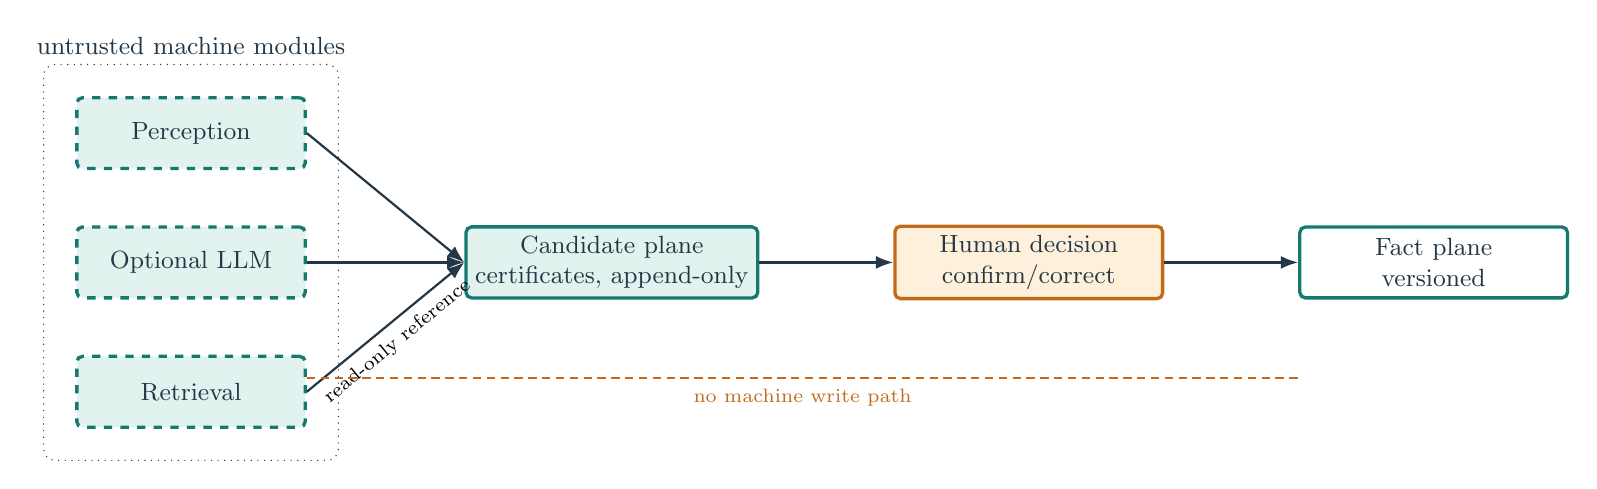
\begin{tikzpicture}[node distance=7mm and 8mm,font=\small]
  \node[machine,minimum width=29mm] (perception) {Perception};
  \node[machine,minimum width=29mm,below=of perception] (llm) {Optional LLM};
  \node[machine,minimum width=29mm,below=of llm] (retrieval) {Retrieval};
  \node[trustbox,minimum width=34mm,right=20mm of llm] (candidate) {Candidate plane\\certificates, append-only};
  \node[human,minimum width=34mm,right=17mm of candidate] (decision) {Human decision\\confirm/correct};
  \node[fact,minimum width=34mm,right=17mm of decision] (fact) {Fact plane\\versioned};
  \draw[flow] (perception.east) -- (candidate.west);
  \draw[flow] (llm.east) -- (candidate.west);
  \draw[flow] (retrieval.east) -- node[below,sloped,font=\scriptsize]{read-only reference} (candidate.west);
  \draw[flow] (candidate) -- (decision);
  \draw[flow] (decision) -- (fact);
  \draw[noflow] ([yshift=-10mm]llm.south east) -- node[below,font=\scriptsize,text=TrustAmber]{no machine write path} ([yshift=-10mm]fact.south west);
  \node[draw=TrustCharcoal,dotted,rounded corners,fit=(perception)(retrieval),inner sep=4mm,label={[text=TrustCharcoal]above:untrusted machine modules}] {};
\end{tikzpicture}}
  \caption{Trust model. Dashed machine components terminate at append-only candidates or read-only references; an attributable human decision is the only exposed path to a versioned fact.}
  \label{fig:trust-model}
\end{figure}

For a recognition input $x$, a predictor returns a class $\hat y(x)$ and a selection score $s(x)$. Given threshold $\tau$, the selection function is
\begin{equation}
  a_\tau(x)=\mathbb{1}[s(x)\geq\tau].
\end{equation}
For a sample of $n$ labeled cases, coverage and selective risk are
\begin{align}
  \widehat{\mathrm{cov}}(\tau)&=\frac{1}{n}\sum_{i=1}^{n}a_\tau(x_i),\\
  \widehat{R}(\tau)&=\frac{\sum_{i=1}^{n}a_\tau(x_i)\mathbb{1}[\hat y_i\neq y_i]}{\max(1,\sum_{i=1}^{n}a_\tau(x_i))}.
\end{align}
The erroneous auto-pass rate uses all cases in the denominator. These empirical measures characterize the recognition gate; they do not alter the authority rule. An accepted recognition is still a candidate, not a fact.

The desired properties are: (P1) machine isolation, Equation~\ref{eq:invariant}; (P2) append-only candidate and fact histories whose candidates are content-addressed certificates; (P3) optimistic concurrency, so a stale decision cannot overwrite a newer version; (P4) content-addressed evidence and reverse trace from export to its supporting chain, rebuilt per field as evidence--certificate--decision--transition with any tampered or missing binding reported as incomplete; and (P5) graceful operation when the optional AI adapter is disabled.

\section{System and methodology}
\label{sec:method}

\subsection{Template-guided perception}
Each form template carries a QR payload identifying its template and version and four ArUco corner markers. The system decodes the QR, estimates a homography from detected corners, warps the image to a canonical canvas, and crops fields from versioned template coordinates. This converts a whole-page task into typed cell decisions and preserves the transformation parameters with the recognition attempt.

Digit crops are resized to $48\times64$ pixels. The built-in comparator binarizes them with Otsu's method and measures normalized mean absolute difference from ten rendered templates. If $d_1(x)$ and $d_2(x)$ are its best and second-best distances, its selection score is
\begin{equation}
  s(x)=d_2(x)-d_1(x).
\end{equation}
The evaluated whole-form configuration instead uses a HOG descriptor with a $48\times64$ window, $16\times16$ blocks, $8\times8$ cells and stride, and nine orientation bins, followed by a linear support-vector machine. Training uses 240 separately seeded rendered cells (eight seeds, three fonts, and ten digits). Its selection score is the difference between the largest and second-largest decision values. Calibration selected $\tau=0$, so all evaluation predictions were retained; the candidate--fact boundary still requires review before a prediction becomes authoritative. OMR cells use an interior fill ratio: at most 0.15 is unchecked, at least 0.35 is checked, and the interval between them is rejected for review.

\begin{figure}[t]
  \centering
  \resizebox{0.96\textwidth}{!}{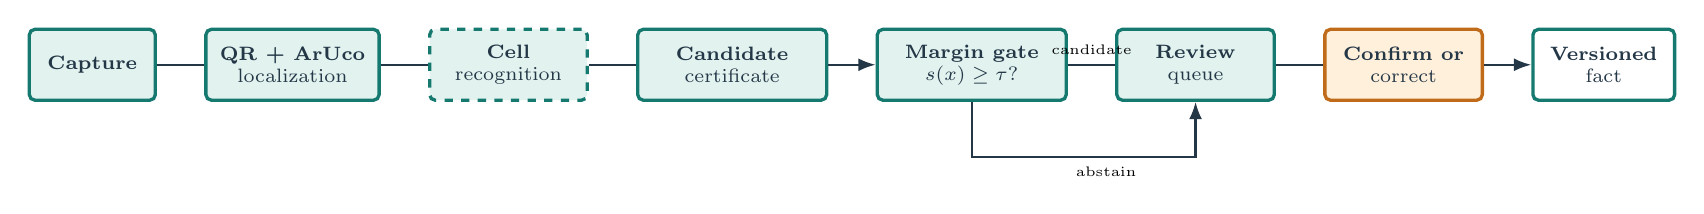
\begin{tikzpicture}[node distance=5mm and 6mm,font=\scriptsize]
  \node[trustbox,minimum width=16mm] (capture) {\textbf{Capture}};
  \node[trustbox,minimum width=22mm,right=of capture] (locate) {\textbf{QR + ArUco}\\localization};
  \node[machine,minimum width=20mm,right=of locate] (recognize) {\textbf{Cell}\\recognition};
  \node[trustbox,minimum width=24mm,right=of recognize] (cert) {\textbf{Candidate}\\certificate};
  \node[trustbox,minimum width=24mm,right=of cert] (gate) {\textbf{Margin gate}\\$s(x)\geq\tau$?};
  \node[trustbox,minimum width=20mm,right=of gate] (queue) {\textbf{Review}\\queue};
  \node[human,minimum width=20mm,right=of queue] (review) {\textbf{Confirm or}\\correct};
  \node[fact,minimum width=18mm,right=of review] (export) {\textbf{Versioned}\\fact};
  \draw[flow] (capture)--(locate)--(recognize)--(cert)--(gate);
  \draw[flow] (gate)--node[above,font=\tiny]{candidate}(queue)--(review)--(export);
  \draw[flow] (gate.south) -- ++(0,-7mm) -| node[pos=.3,below,font=\tiny]{abstain} (queue.south);
\end{tikzpicture}
}
  \caption{Operational pipeline. Recognition outcomes cross the threshold gate into the review queue but remain non-authoritative until a confirm/correct action.}
  \label{fig:pipeline}
\end{figure}

\subsection{Candidate, decision, and fact services}
Evidence is assigned a SHA-256 digest. Recognition attempts and AI reviews are stored independently from confirmed record versions. The optional AI adapter accepts structured context and must return schema-valid review JSON; its prompt contract states that it cannot modify business facts. The default adapter is disabled, returning an explicit \texttt{NOT\_RUN} status. Local retrieval uses a dependency-free similarity index and exposes results only as references.

The review service accepts an expected record version, reviewer identifier, reason, candidate values, and evidence identifiers. It rejects a stale expected version, appends a new confirmed record on success, and emits a corresponding audit event. Exports query confirmed records only. Figure~\ref{fig:lineage} shows the reverse-trace chain.

\begin{figure}[t]
  \centering
  \resizebox{0.96\textwidth}{!}{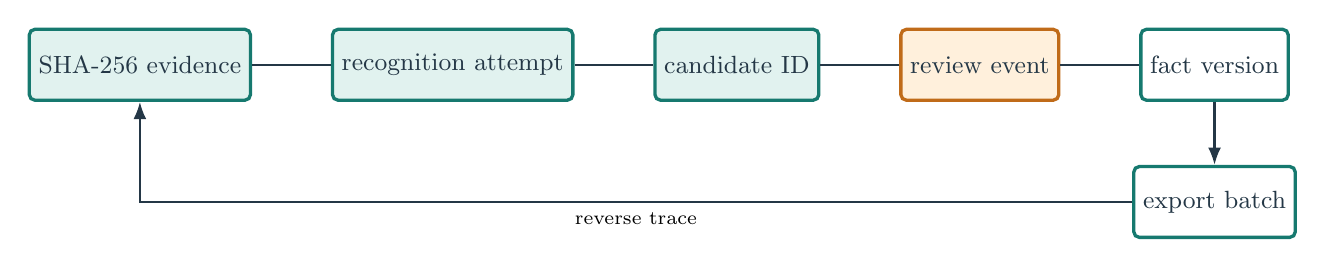
\begin{tikzpicture}[node distance=8mm and 10mm,font=\small]
  \node[trustbox] (hash) {SHA-256 evidence};
  \node[trustbox,right=of hash] (attempt) {recognition attempt};
  \node[trustbox,right=of attempt] (candidate) {candidate ID};
  \node[human,right=of candidate] (event) {review event};
  \node[fact,right=of event] (version) {fact version};
  \node[fact,below=of version] (batch) {export batch};
  \draw[flow] (hash)--(attempt)--(candidate)--(event)--(version)--(batch);
  \draw[flow] (batch.west) -| node[pos=.25,below,font=\scriptsize]{reverse trace} (hash.south);
\end{tikzpicture}
}
  \caption{Evidence lineage from content-addressed input to export. Every arrow represents a persisted identifier used by the reverse-trace check.}
  \label{fig:lineage}
\end{figure}

\subsection{Implementation}
The evaluated artifact is a local single-machine prototype implemented with Python~3.11, Streamlit, SQLite, SQLAlchemy, Alembic, OpenCV, scikit-learn, and an optional provider adapter. Domain, application, adapter, and user-interface layers separate fact-transition services from machine-facing services. The experiment harness invokes these same repositories and application services for import, candidate persistence, confirmation, export, and trace queries.

The system retains local evidence, database, and export files as one backup unit. This local-first operational choice supports recovery in a small-plant setting \citep{kleppmann2019}, but it is not itself a security boundary. Deployment still requires host access control, encrypted backups, retention rules, and tested restore procedures.

\section{Experimental protocol}
\label{sec:protocol}

\subsection{Research questions}
The evaluation addresses three questions. \textbf{RQ1} asks how risk-targeted abstention changes coverage and error exposure. \textbf{RQ2} asks whether injected machine and workflow faults can change an existing fact through exposed application paths. \textbf{RQ3} asks whether core import--review--export operations, provenance, and concurrency checks remain functional without the AI adapter and across repeated executions.

\subsection{Synthetic recognition benchmark}
Production forms can contain employee identifiers, payroll-adjacent values, and commercially sensitive production data. They were therefore neither used in the public benchmark nor sent to external AI services. Instead, the package deterministically renders synthetic form cells with known labels. This decision makes the benchmark distributable and repeatable but limits ecological validity.

The benchmark contains 4,350 image rows. Seeds 101 and 202 define 1,740 calibration rows; disjoint seeds 303, 404, and 505 define 2,610 evaluation rows. The evaluation split contains 90 seed--font--digit base units, each observed under 29 clean or perturbed conditions. Consequently, rows are disjoint from calibration by seed but are not mutually independent within the evaluation split. Training data for the learned baseline use separate seeds. Perturbations comprise clean images plus Gaussian blur, Gaussian noise, brightness reduction, rotation, perspective distortion, JPEG compression, and occlusion at predefined severities. The implementation records every raw prediction, score, label, model, perturbation, severity, and seed.

Thresholds from 0 to 0.10 are swept in increments of 0.005. The operating threshold is selected \emph{only on calibration rows} as the lowest threshold in the grid satisfying a target empirical selective risk of at most 1\%, thereby retaining the highest calibration coverage among qualifying thresholds. The selected value is then frozen for evaluation. We report coverage, accepted accuracy, selective risk, erroneous auto-pass rate, and routing rate. The generated table also includes a descriptive row-level Wilson interval for accepted accuracy. Because that interval assumes independent Bernoulli trials whereas perturbations reuse base units, it is not treated as cluster-valid inferential evidence.

Three available recognition paths are compared: the Auto-Decte template matcher, the same template decision forced to predict whenever possible, and a HOG feature extractor with a linear support-vector machine. A Tesseract path is capability-gated. The executable was unavailable in the recorded environment, so no Tesseract score is reported.

\subsection{Fault injection and resilience}
Five application-path faults probe distinct boundaries: a wrong recognition candidate, a wrong language-model suggestion, an irrelevant retrieval result, a stale human-review replay, and duplicate evidence. A run passes only when the existing fact remains unchanged and an audit outcome is recorded; stale review and duplicate evidence must additionally raise their designated exceptions.

Resilience checks exercise import, human confirmation, export, reverse trace, duplicate rejection, stale-version rejection, and operation with AI disabled. Latency is measured over 30 repetitions after five warm-ups for both fresh-container (cold) and reused-container (warm) application flows. These sub-millisecond service timings exclude image decoding, browser rendering, storage-device variance, and human review, and therefore should not be interpreted as end-to-end user latency.

\subsection{Reproducibility controls}
The experiment code fixes seeds and dependency versions, emits JSON before figures or tables, and writes a manifest containing SHA-256 hashes, commands, environment metadata, source commit, and working-tree status. Paper tables are generated from the same JSON read by the plots. The final code quality gate comprises unit/integration tests, Ruff static checks, and mypy type checks. The evaluation is synthetic by design; a production claim would require a separate, access-controlled protocol with double transcription and adjudication.

\section{Results}
\label{sec:results}

\subsection{RQ1: recognition and selective risk}
The template matcher required a conservative operating point. Calibration selected $\tau=0.08$; on the 2,610 evaluation rows, it accepted 292 predictions and routed 2,318 to review. Coverage was 11.19\% (cluster-bootstrap 95\% interval 5.86\%--16.97\%), with no accepted error observed. The corresponding cluster-bootstrap interval for accepted accuracy was 100\%--100\%; this degenerate interval reflects the deterministic sample and does not establish a zero population error rate.

The HOG--linear-SVM changed the operating trade-off. Its calibration split already met the 1\% risk target at $\tau=0$, so the frozen selector accepted all 2,610 evaluation rows. It correctly classified 2,605, giving 99.81\% accepted accuracy and 0.19\% selective risk. Cluster resampling placed the risk interval at 0.038\%--0.346\% and the accepted-accuracy interval at 99.62\%--99.96\% (Table~\ref{tab:selective-models}). The result supports HOG--SVM as the evaluated digit recognizer; it does not support a claim of recognition novelty.

\begin{table}[t]
  \centering
  \caption{Calibration-selected operating points on the seed-disjoint evaluation split. Confidence intervals reported in the text resample 90 base units rather than 2,610 rows.}
  \label{tab:selective-models}
  \begingroup
  \footnotesize
  \setlength{\tabcolsep}{3pt}
  \begin{tabular}{lrrrr}
\toprule
Model & Cov. (\%) & Acc. (\%) & Risk (\%) & Review (\%) \\
\midrule
Template matcher & 11.2 & 100.00 & 0.00 & 88.8 \\
HOG--SVM & 100.0 & 99.81 & 0.19 & 0.0 \\
\bottomrule
\end{tabular}

  \endgroup
\end{table}

\begin{figure}[t]
  \centering
  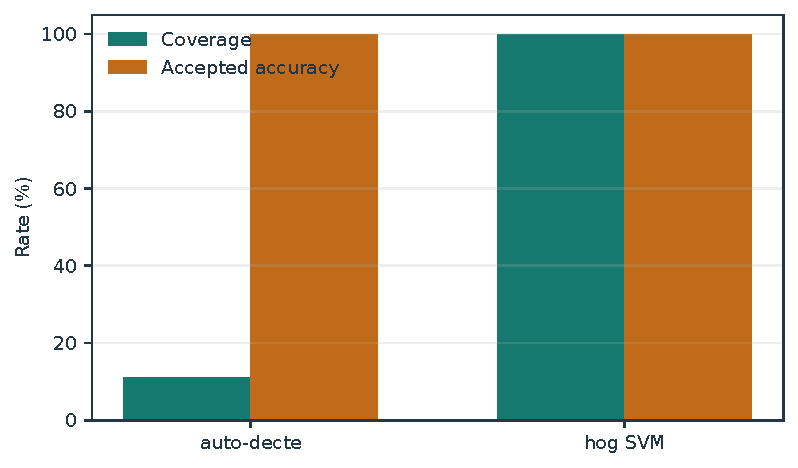
\includegraphics[width=0.76\textwidth]{figures/generated/model_selective_comparison.pdf}
  \caption{Coverage and conditional accepted accuracy for the two calibration-selected recognizer--gate combinations.}
  \label{fig:selective-models}
\end{figure}

The template gate remains informative as a stress case. Figure~\ref{fig:coverage-risk} shows that its full-coverage end incurred roughly 25\% selective risk; the first threshold with zero observed accepted error was $\tau=0.07$, at 14.83\% coverage. Severe perspective distortion and occlusion reduced its coverage to 3.33\%. Thus, selection prevented many weak template predictions from auto-passing, but the stronger HOG representation removed most of that synthetic-regime trade-off.

\begin{figure}[t]
  \centering
  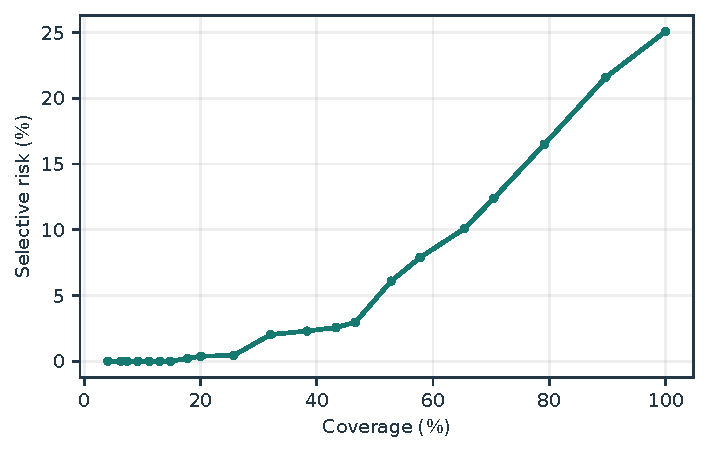
\includegraphics[width=0.76\textwidth]{figures/generated/coverage_risk.pdf}
  \caption{Template-matcher coverage--risk curve. The dashed operating point was selected on calibration data before evaluation.}
  \label{fig:coverage-risk}
\end{figure}

\subsection{RQ2: whole-form integration}
Across the 300 evaluation form--condition rows, template identification succeeded on 80\% and ArUco alignment succeeded on 80\%; both succeeded together on 180 rows (60\%). Across all conditions, digit accuracy was 86.03\%, OMR accuracy was 100\%, and complete-form success was 60\% (Table~\ref{tab:whole-form}). All 60 clean, 60 perspective, and 60 JPEG rows were completely correct. Gaussian blur preserved alignment and 100\% field accuracy but prevented QR identification on all 60 rows. Rotation preserved QR identification but prevented marker alignment on all 60 rows and reduced digit accuracy to 30.17\%. These complementary failures explain why the two marginal component rates exceed their joint rate and why the complete endpoint is 60\%.

\begin{table}[t]
  \centering
  \caption{Whole-form evaluation over 300 form--condition rows per variant. Complete success requires template identity, alignment, and all 20 fields correct.}
  \label{tab:whole-form}
  \begingroup
  \footnotesize
  \setlength{\tabcolsep}{3pt}
  \begin{tabular}{lrrrrr}
\toprule
Variant & QR (\%) & Align (\%) & Digit (\%) & OMR (\%) & Complete (\%) \\
\midrule
full\_pipeline & 80.0 & 80.0 & 86.0 & 100.0 & 60.0 \\
without\_qr & 0.0 & 80.0 & 86.0 & 100.0 & 0.0 \\
without\_aruco & 80.0 & 0.0 & 69.4 & 99.0 & 0.0 \\
\bottomrule
\end{tabular}

  \endgroup
\end{table}

Suppressing QR identification left field recognition unchanged but made the complete endpoint unattainable. Suppressing ArUco alignment reduced digit accuracy from 86.03\% to 69.43\% and OMR accuracy from 100\% to 99.03\%; complete-form success again fell to zero. Figure~\ref{fig:whole-form} separates the component rates so the endpoint's conjunctive definition is explicit.

\begin{figure}[t]
  \centering
  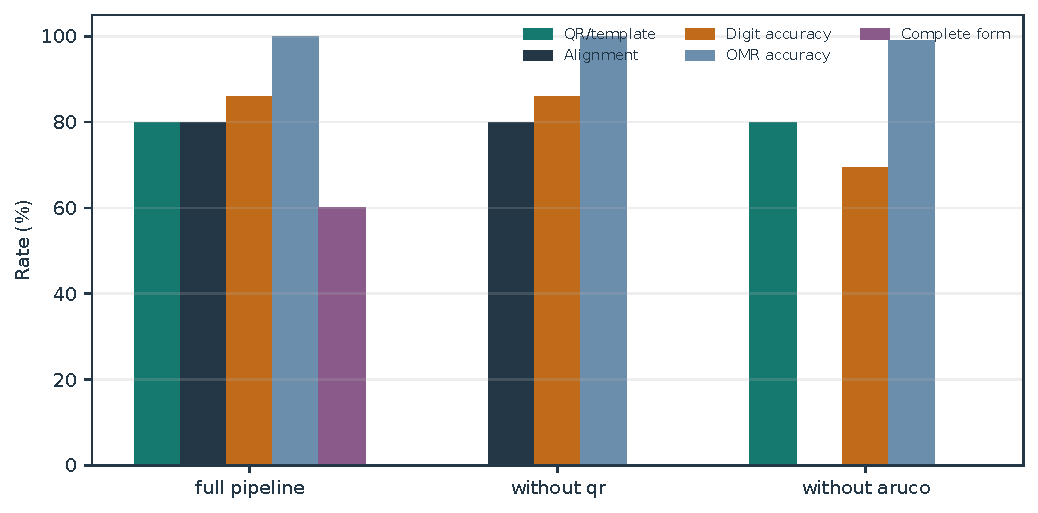
\includegraphics[width=0.82\textwidth]{figures/generated/whole_form_ablation.pdf}
  \caption{Whole-form component ablations. Removing a component required by the endpoint forces complete success to zero; field metrics show the additional recognition effect of missing alignment.}
  \label{fig:whole-form}
\end{figure}

\subsection{RQ3: authority-boundary faults}
All six controlled cases left the pre-existing fact unchanged and produced complete audit evidence. Wrong recognition and language-model outputs remained candidates, irrelevant retrieval remained a reference, stale review and duplicate evidence raised their designated exceptions, and all 12 attempted direct fact-write paths were absent from the three machine-facing services.

The candidate-isolation ablation supplied an incorrect value of 999. Under normal wiring, recording the candidate did not change the fact. Under test-only unsafe wiring that granted the same value access to the review service, the fact changed. This contrast locates containment in capability separation rather than in the injected value or recognizer behavior.

Randomized stress testing repeated five fault families 100 times each. All 500 trials were contained (Table~\ref{tab:fault-stress}). This expands the evidence beyond one example per family, although it remains an application-path test rather than a penetration test, formal proof, or assessment of host compromise.

\begin{table}[t]
  \centering
  \caption{Seeded randomized trust-boundary stress test.}
  \label{tab:fault-stress}
  \begin{tabular}{lrr}
\toprule
Fault family & Contained & Trials \\
\midrule
wrong\_recognition & 100 & 100 \\
wrong\_llm\_suggestion & 100 & 100 \\
irrelevant\_retrieval & 100 & 100 \\
stale\_human\_replay & 100 & 100 \\
duplicate\_evidence & 100 & 100 \\
\bottomrule
\end{tabular}

\end{table}

\subsection{RQ4: executable workflow and reproducibility}
Each of the 60 clean evaluation forms traversed the complete application workflow. The runner imported the original image, stored 20 recognition candidates, programmatically submitted known synthetic labels through the review service, created fact version~1, exported an XLSX file, and queried the reverse trace. All 60 workflows succeeded, accounting for 1,200 persisted candidate attempts. This verifies the software path but not human-review effectiveness. AI-disabled operation, duplicate rejection, stale-version rejection, and reverse tracing also passed.

The final verification run passed 77 automated tests, Ruff checks, and mypy checks. The artifact manifest contains 27 hashed outputs, records source commit \texttt{195355a}, and reports a clean tracked source state at generation time. Service microbenchmarks and the full perturbation table are supplied in the supplementary material because they do not measure end-to-end reviewer latency.

\section{Industrial context and intended use}
\label{sec:context}

The system was motivated by paper-based production records in a bamboo-processing setting, where form values can be adjacent to employee identity, output accounting, and payroll decisions. The intended user is a reviewer who receives a digitized form, inspects machine candidates alongside image evidence, confirms or corrects values, and exports only confirmed records. The prototype demonstrates that this workflow can be represented in software, but the paper does not claim a measured deployment effect on cost, time, accuracy, wages, or organizational outcomes.

No production-form corpus was available to this study under an authorized research-use protocol. We therefore used deterministic synthetic forms for controlled and reproducible mechanism evaluation. Privacy, commercially sensitive content, and authorization requirements further constrain the acquisition and public release of such data. Synthetic forms preserve known labels, controlled perturbations, and distributable evidence. They do not reproduce handwriting variation, capture habits, paper wear, device diversity, or reviewer behavior in the plant.

For production adoption, the authority model should be embedded in a broader control system: least-privilege host access, encrypted storage and backups, retention schedules, separation of reviewer and payroll roles where required, audit review, incident response, and periodic sampling of confirmed records. Candidate--fact separation reduces one route by which machine error becomes operational truth; it does not replace these organizational controls.

\section{Discussion}
\label{sec:discussion}

The experiments distinguish predictive performance from governance performance. HOG--SVM reduced cell error to 0.19\% in the synthetic evaluation, but five mistakes remained. The authority boundary addresses the destination of such errors: even a selected prediction is persisted as a candidate until an attributable, version-checked review creates a fact. Stronger perception therefore reduces reviewer workload without making candidate--fact separation redundant.

Recognizer choice also changed the role of selective prediction. The template matcher needed to route 88.81\% of evaluation rows to achieve zero observed accepted errors, whereas HOG--SVM satisfied the calibration risk target at full coverage. This difference argues against treating a threshold as a fixed safety setting. Selection must be recalibrated after changes in forms, printers, cameras, or recognizers, and a deployment threshold should reflect the relative cost of an unreviewed error, reviewer time, and delayed processing.

The whole-form benchmark exposed failures that the cell benchmark could not. Digit and OMR recognition were perfect under blurred forms once fields were localized, yet QR identification failed, so no complete record could be produced. Under rotation, ArUco alignment failed and digit accuracy fell sharply. These observations make the engineering priorities concrete: QR preprocessing or fallback classification is needed for blur, and marker detection or orientation normalization is needed for rotation. The 60\% complete-form result is consequently more informative than the 99.81\% isolated-cell score for the current pipeline.

The controlled fault cases, candidate-isolation ablation, and 500 randomized trials test the causal role of capability separation. The incorrect value was harmless when stored through a candidate-only interface and changed the fact when the experiment deliberately exposed the review capability. This is stronger evidence than an architecture diagram alone, but weaker than formal noninterference verification, database privilege separation, or adversarial assessment of every UI and migration path.

The authority-integration benchmark tests the boundary in its executable form. Certificates bind a candidate to its field, evidence, and expected version, so a certificate moved to another field or confirmed against another form's evidence is rejected before any write. Confirmations commit per-field decisions, transitions, and the record version in one compare-and-swap transaction, so concurrent and stale confirmations fail closed. Reverse traces are rebuilt from the database per field rather than assumed, and the benchmark shows that tampered producers, deleted transitions, and record-version rebinding---including rebinding to another existing row that the database foreign key still accepts---are reported as incomplete. The measured silent fault escape of 0.75 belongs to the scripted reviewer and is deliberately not interpreted as human error rates; that question is deferred to the controlled human-review study.


The architecture remains model-agnostic. A conformal or learned selector can replace the decision-margin rule, and different retrieval or language models can supply assistance, provided that each terminates outside the fact-writing interface. This separation allows model procurement to change while preserving a stable audit question: which service can invoke the fact-transition operation?

The next empirical study should use a blinded, double-entered corpus of real forms with adjudicated ground truth and subgroup reporting by template, device, writing style, and degradation. A second study should randomize review interfaces---recognition only, retrieval-assisted, and AI-assisted---and measure review time, correction accuracy, automation bias, and inappropriate suggestion acceptance. Those studies would test decision quality and operational value, which synthetic execution cannot establish.

\section{Limitations and threats to validity}
\label{sec:limitations}

\textbf{External validity.} All quantitative recognition results use deterministic synthetic cells. They do not represent handwriting, Chinese text, signatures, paper damage, camera diversity, or the joint distribution of production forms. The privacy rationale for withholding production data is legitimate, but it does not turn synthetic evidence into field evidence.

\textbf{Statistical validity.} Threshold selection uses a disjoint calibration split, reducing direct evaluation leakage. Nevertheless, calibration and evaluation arise from the same renderer and perturbation generator. Zero observed accepted errors among 292 cases produces a Wilson lower bound of 98.70\%, not proof of perfect accuracy. Perturbation-level groups contain 90 cases and therefore support only coarse comparisons.

\textbf{Construct validity.} The trust tests operationalize containment as an unchanged fact plus complete audit evidence. This captures the stated application invariant but not human susceptibility to misleading suggestions, correctness of a later human decision, confidentiality, availability, or resistance to host compromise. ``Trust-constrained'' should not be read as a general security certification.

\textbf{Baseline validity.} The HOG--SVM baseline is strong on this renderer and may benefit from the constrained visual regime. Conversely, Tesseract was not installed and was excluded rather than simulated. Broader OCR and document-model comparisons on real data remain necessary.

\textbf{Implementation scope.} The evaluated prototype is local and single-machine, with a Streamlit interface. It has not been load-tested for concurrent users and does not yet implement production authentication or role-based access. Sub-millisecond service timings are microbenchmarks, not end-to-end latency.

\textbf{Reproducibility.} Seeds, code, raw predictions, summary JSON, plots, tables, and hashes are supplied. Reproduction still depends on compatible OpenCV and system behavior, and independent execution has not yet been reported. The public package intentionally excludes sensitive plant records.

\section{Conclusion}
\label{sec:conclusion}

Auto-Decte treats machine outputs as evidence-linked candidates rather than authoritative facts. Within the exposed application services, perception, retrieval, and optional language-model review have no direct fact-writing path; a version-checked, attributable human decision over a content-addressed certificate is required. HOG--SVM achieved 99.81\% cell accuracy, but the full pipeline completed only 60\% of perturbed whole forms because blur defeated QR identity and rotation defeated marker alignment. In the integrated system, confirmations commit per-field decisions, transitions, and the record version in one compare-and-swap transaction, and reverse traces rebuilt from the database reported every injected corruption---tampered producers, deleted transitions, and record-version rebinding---as incomplete. All 60 clean evidence-to-export workflows were traceable, 12 direct-write attempts were unavailable, and 500 randomized faults were contained without changing existing facts.

The evidence supports the feasibility of the architecture and its executable invariants, not production effectiveness or universal safety. Real-form validation and controlled human-review studies are the necessary next steps. The central design lesson is portable: improve models when possible, but design the data path so that model confidence is never confused with authority.
\section*{Declarations}

\textbf{Data and code availability.} The reproducible synthetic benchmark, raw predictions, summary artifacts, figure-generation code, and application source are included in the accompanying repository. Production forms are not included because they may contain employee identity, payroll-adjacent values, and commercially sensitive production information.

\textbf{Declaration of generative AI and AI-assisted technologies in the manuscript preparation process.} During the preparation of this work, the authors used DeepSeek Harness and OpenAI Codex to assist with drafting, content organization, language editing, and AI-assisted code development. The authors reviewed, edited, and verified the resulting text, code, analyses, references, and claims, and take full responsibility for the content of the publication. No generative-AI-created or generative-AI-altered image is included in this submission; diagrams are author-controlled vector graphics and quantitative plots are generated programmatically from the reported experiment artifacts.

\textbf{Funding, competing interests, and author contributions.} These items remain for the authors to complete with verified information before submission; they are omitted from this author-redacted technical review copy.


\bibliographystyle{elsarticle-harv}
\bibliography{references}

\end{document}
